\section{Durchführung}
\label{sec:Durchführung}

% Was wurde gemessen bzw. welche Größen wurden variiert?
Eine Drillachse wird wie in \autoref{fig:aufbau} aufgebaut.

\begin{figure}
    \centering
    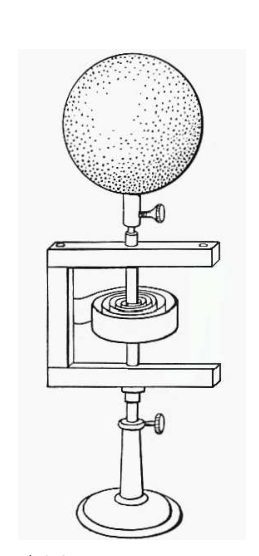
\includegraphics[height=8cm]{images/aufbau.png}
    \caption{Darstellung einer Drillachse für das beschriebene Experiment \cite{V101}}
    \label{fig:aufbau}
\end{figure}

Zunächst wird die Winkelrichtgrößte $D$ bestimmt. 
Dafür wird eine Federwaage und eine annähernd masselose Stange verwendet.
Die Stange wird auf der Drillachse fixiert und die Federwaage in die Stange eingehakt. 
Der Abstand von der Rotationsachse bis zum Punkt, an dem die Federwaage eingehakt ist, wird gemessen.
Nun wird das System um einen Winkel $\varphi$ ausgelenkt. 
An der Federwaage wird eine Kraft $F$ abgelesen und in Abhängigkeit von $\varphi$ notiert. 
Diese Messung wird mindestens zehn mal für verscihedene Auslenkungen durchgeführt. 
Aus dem Zusammenhang \autoref{eq:winkelrichtgroesse} lässt sich $D$ bestimmen.

Für die Bestimmung des Eigenträgheitsmoments $I_\text{D}$ der Drillachse wird erneut eine als masselos anzunehmende Stange verwendet, sowie zwei Gewichte.
Diese Gewichte werden in einem Abstand $a$ von der Rotationsachse an der Stange befestigt und um einen kleinen Winkel $\varphi$ ins Schwingen gebracht. 
Daraus lässt sich mit einer Stoppuhr die Periodendauer $T$ bestimmen. 
Diese Messung wird für mindestens zehn verschiedene Abstände $a$ wiederholt. 

Im eigentlichen Versuch wird jetzt das Trägheitsmoment zwei verschiedener Körper experimentell bestimmt. 
Dafür werden alle verwendeten Körper ausgemessen und ihre Masse $m$ bestimmt. 
Dann wird je ein Körper auf der Drillachse befestigt. 
Das Vorgehen ist ähnlich wie zuvor. 
Der Körper wird für kleine Winkel $\varphi$ ausgelenkt und zum Schwingen gebracht. 
Mit einer Stoppuhr wird die Periodendauer $T$ mindestens fünf mal bestimmt. 
Dieser Vorgang wird für insgesamt zwei verschiedene Körper durchgeführt.

Im letzten Versuchsteil werden erneut zwei Trägheitsmomente bestimmt. Dafür wird eine Puppe verwendet.
Diese wird in zwei verschiedene Stellungen gebracht, siehe \autoref{fig:puppe1} und \autoref{fig:puppe2}. 
Durch das oben beschriebene Verfahren wird das entsprechende Trägheitsmoment $I$ dieser Stellung bestimmt. 
Die Puppe wird wieder zum Schwingen gebracht, wobei die Periodendauer $T$ mit einer Stoppuhr gemessen wird.
Außerdem wird die Puppe mit Zylindern angenähert und die Durchmesser und die Längen dieser Zylinder werden vermessen bzw. abgeschätzt.

\begin{figure}
    \centering
    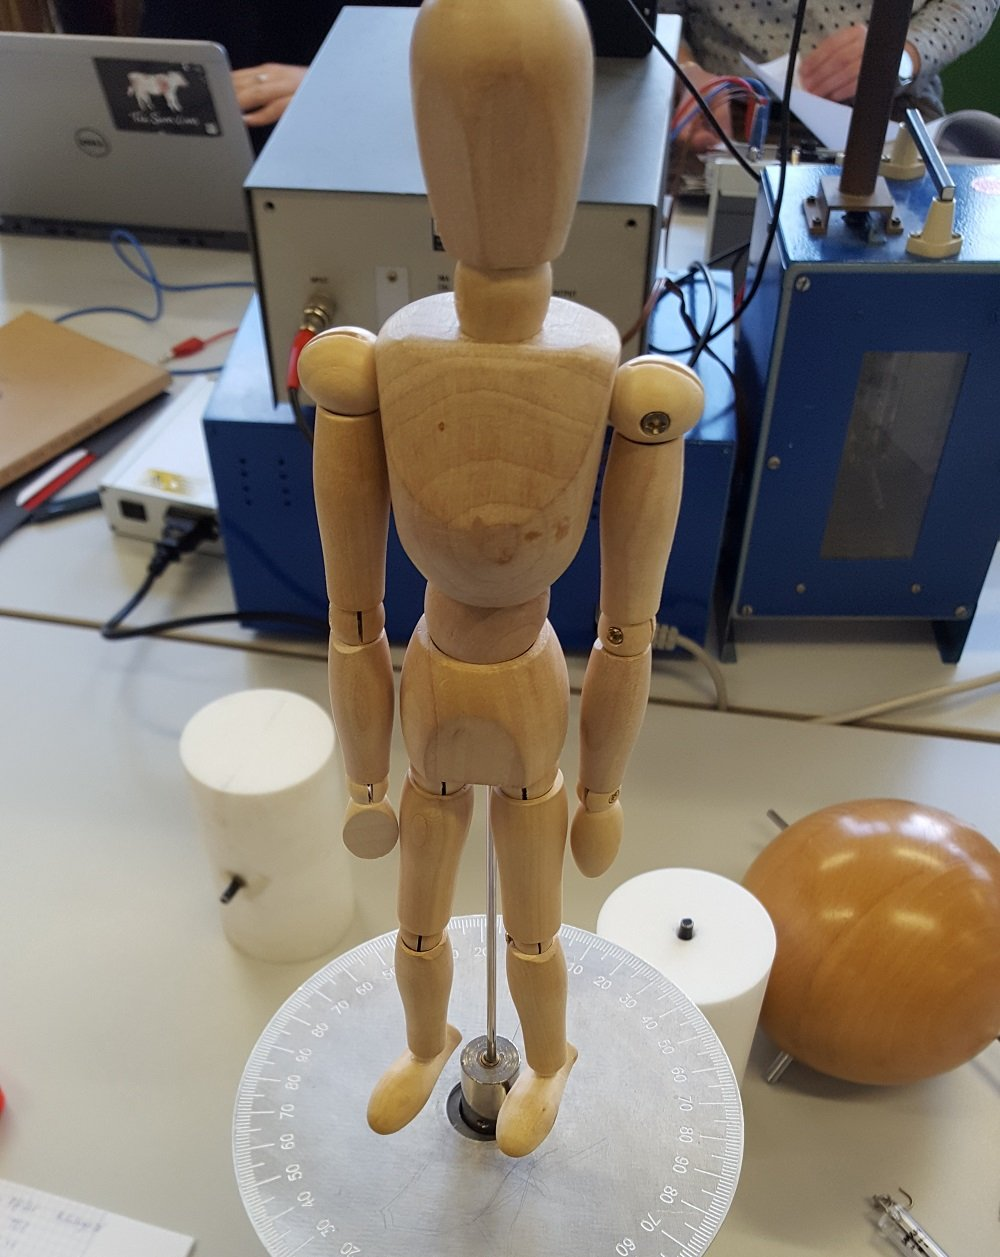
\includegraphics[height=7.5cm]{images/foto_7.jpg}
    \caption{Darstellung der verwendeten Puppe in Stellung 1 \cite{V101}}
    \label{fig:puppe1}
\end{figure}

\begin{figure}
    \centering
    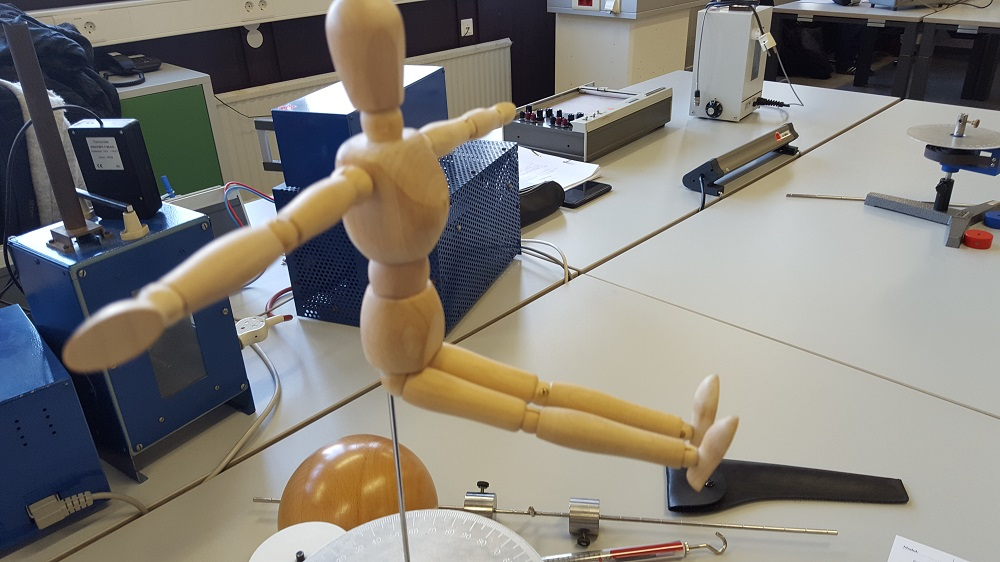
\includegraphics[height=6cm]{images/foto_9.jpg}
    \caption{Darstellung der verwendeten Puppe in Stellung 2 \cite{V101}}
    \label{fig:puppe2}
\end{figure}